
\subsection{MPS}

A general quantum state with n sites can be described in a given basis $\ket{i}$ as
\begin{equation}
    \ket{\Psi} = \sum_{i_1 i_2 \cdots i_n } C^{i_1 i_2 \cdots i_n} \ket{i_1} \otimes \ket{i_2} \otimes \cdots \otimes \ket{i_n}
\end{equation}

This requires an exponential number $d^n$ of coefficients C where d is the dimensions of basis $\ket{i}$.





In order to make the problem tractable, the following form is proposed as wavefunction:

\begin{equation}
    C^{i_1 i_2 \cdots i_n} = {C^{1}}_{\alpha_1}^{ i_1} {C^{2}}_{\alpha_1 \alpha_2}^{i_2} \cdots  {C^{n}}_{\alpha_{n-1} }^{i_n}
\end{equation}
Where summation over shared indices is implied. It is always possible to find such an representation by means of matrix decomposition. The summation over $\alpha_i$ are called virtual bond and their dimension is denoted by $\chi$.


\begin{figure}
    \centering

    \begin{tikzpicture}[ ]

        \draw (-3,-0) rectangle (1,1)  [add reference=C]   ;
        \node  at (C center) {C};


        \node (N1)  at  (-2.5,-1) {};
        \node (N2)  at  (-1.5,-1) {};
        \node  at  (-.5,-0.5) {...};
        \node  (N3) at  (.5,-1) {};


        \draw    (N1) -- (N1 |-  C south);
        \draw    (N2) -- (N2 |-  C south);
        \draw    (N3) -- (N3 |-  C south);

    \end{tikzpicture}

    \caption{Caption}
    \label{fig:my_label}
\end{figure}



Explicit translational invariance is given by tensor $C^i_{\alpha \beta }$ that don't depend on the location. The chain is closed by setting $\alpha_n = \alpha_0$. We can now write this as a Trace over matrix products:

\begin{equation}
    \ket{\Psi} = \Tr( C^{i_1} C^{i_2} \cdots C^{i_n}  ) \ket{i_1} \otimes \ket{i_2} \otimes \cdots \otimes \ket{i_n}
\end{equation}

\missingfigure{make this in graphical notation}


\subsection{graphical notation}
Tensor networks can be written in a graphical notation. The legs f a tensor denote the number of external indices. The upper  Connected legs are summed. Some examples are shown in \cref{tab:grafical_not}

\begin{table}[]
    \centering
    \caption{Caption}
    \begin{tabular}{l|l|l}
        conventional            & Einstein                & tensor notation           \\
        \hline
        $\Vec{x}$               & $x_{\alpha}$            &

        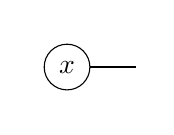
\begin{tikzpicture}[baseline=({N2.base}) ]
            \clip (-0.5,-0.5) rectangle (1,0.5);
            \node[circle, draw] (N2) at (0,0) {$x$};
            \node[] (N1) at (1,0) {};
            \draw  (N1) -- (N2) ;
        \end{tikzpicture}                                                     \\
        M                       & $M_{\alpha \beta}$      & 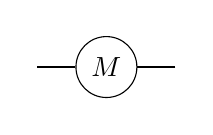
\begin{tikzpicture}[baseline={0cm-0.5*height("$=$")} ]
            \clip (-1,-0.5) rectangle (1,0.5);

            \node[circle, draw] (N2) at (0,0) {$M$};
            \node[] (N0) at (-1,0) {};
            \node[] (N1) at (1,0) {};

            \draw  (N1) -- (N2) ;
            \draw  (N0) -- (N2) ;

        \end{tikzpicture} \\

        $\Vec{x} \cdot \Vec{y}$ & $x_{\alpha} y_{\alpha}$ & 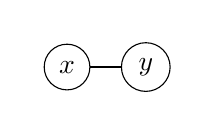
\begin{tikzpicture}[baseline=({N2.base}) ]
            \clip (-0.5,-0.5) rectangle (1.5,0.5);
            \node[circle, draw] (N2) at (0,0) {$x$};
            \node[circle, draw] (N1) at (1,0) {$y$};
            \draw  (N1) -- (N2) ;
        \end{tikzpicture} \\
    \end{tabular}

    \label{tab:grafical_not}
\end{table}





\subsection{MPO}

In a similar fashion, a Matrix Product Operator (MPO) is of the following form:

\begin{equation} \label{def_mpo}
    \begin{split}
        \hat{O} &= \sum Tr(A^{i_1 j_1} A^{i_2 j_2} \cdots A^{i_n j_n} M) \\
        & \times \ket{i_1}\bra{j_1} \otimes \ket{i_2}\bra{j_2} \otimes \cdots \otimes \ket{i_n}\bra{j_n}
    \end{split}
\end{equation}

\mpo{5}{{,,,,,}}{{"$i_1$","$i_2$",,"$i_n$","-"}}{{"$j_1$","$j_2$",,"$j_n$","-"}}{{0,0,1,0,0}}{{"A", "A",,"A","M" }}
\todo{connect trace and hide legs at M}



The matrix M contains the boundary conditions of the operator. Many Hamiltonians can be represented by an MPO. For ins

\subsection{PEPO}